
\documentclass[Midterm2Review_Rec.tex]{subfiles}

\section{Applied Competitive Analysis}

\begin{frame}{Demand and Supply, PS and CS}
	
	\begin{itemize}
		\item Market demand curve: the set of consumers arranged in inverse ordering from the person with the highest willingness to pay (WTP) to the person with the lowest WTP for a commodity. It is aggregated from Marshallian demands.
		\item Market supply curve: the set of producers arranged in order from the firm willing to produce at the lowest price to the firm demanding the highest price to produce a good.
		\item 
		Consumer surplus: the difference between the maximum value that a consumer is willing to pay for a quantity of commodity minus the market price of that quantity of commodity.
		\item Producer surplus: what the producer receives for goods in excess of the cost of production.
		\item 	
		A competitive market maximizes the sum of producer and consumer surplus: all gains from trade are realized; all transactions that benefit both parties occur; no transactions occur that do not benefit both parties.
	\end{itemize}
\end{frame}



\begin{frame}{Demand and CS}
\begin{figure}
	\centering
	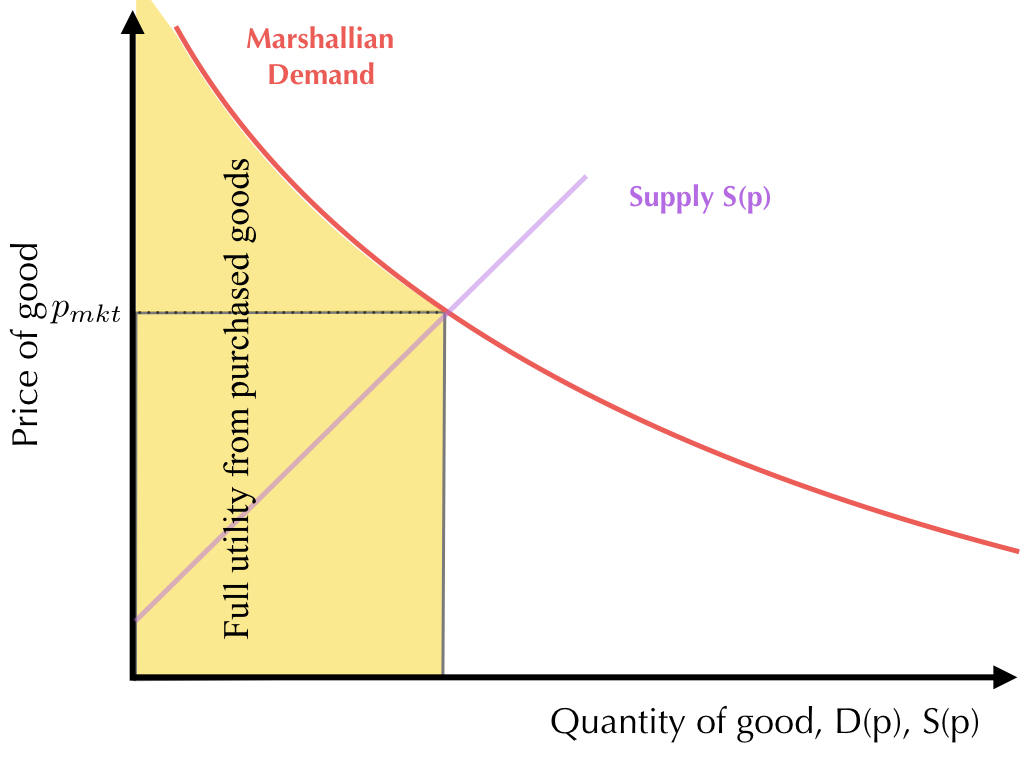
\includegraphics[width=0.5\linewidth]{Figures/CS1}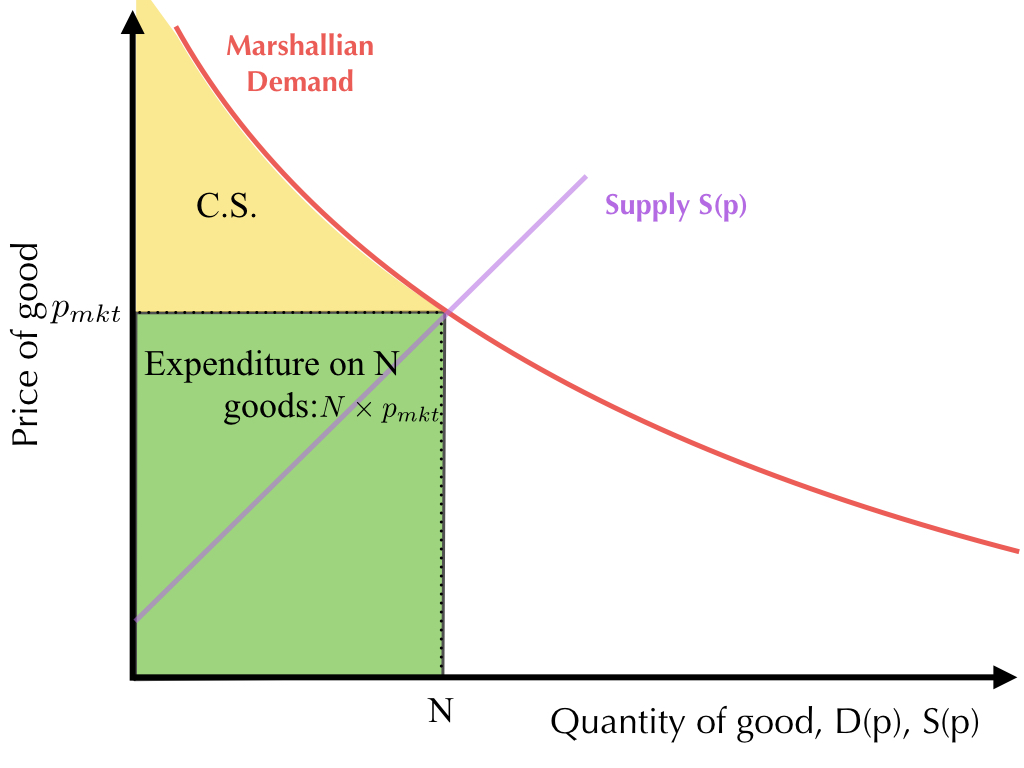
\includegraphics[width=0.5\linewidth]{Figures/CS2}
\end{figure}
	{\footnotesize Left: Demand curve. Each value on the vertical axis is the valuation of marginal units by the consumer. Shaded area is total willingness to pay for all units up to N (utility in dollar terms from consuming N).}\\
{\footnotesize Right:CS is the total willingness to pay for N goods minus the expenditure on those goods.}
\end{frame}



\begin{frame}{Supply and PS}
\begin{figure}
	\centering
	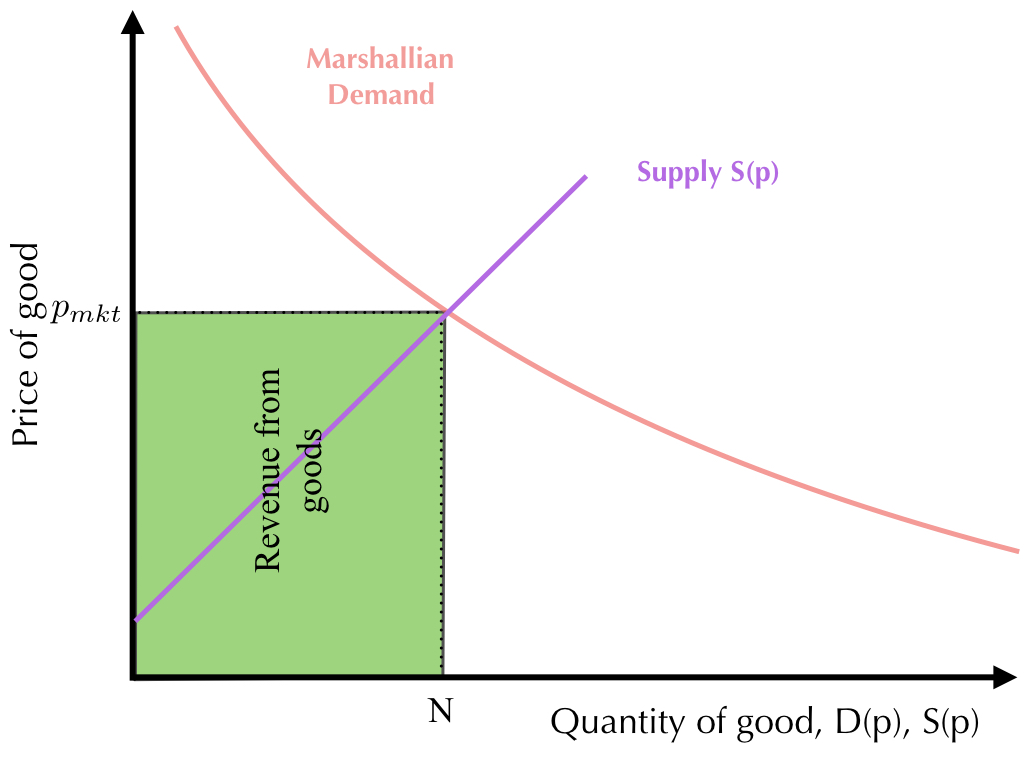
\includegraphics[width=0.5\linewidth]{Figures/PS1}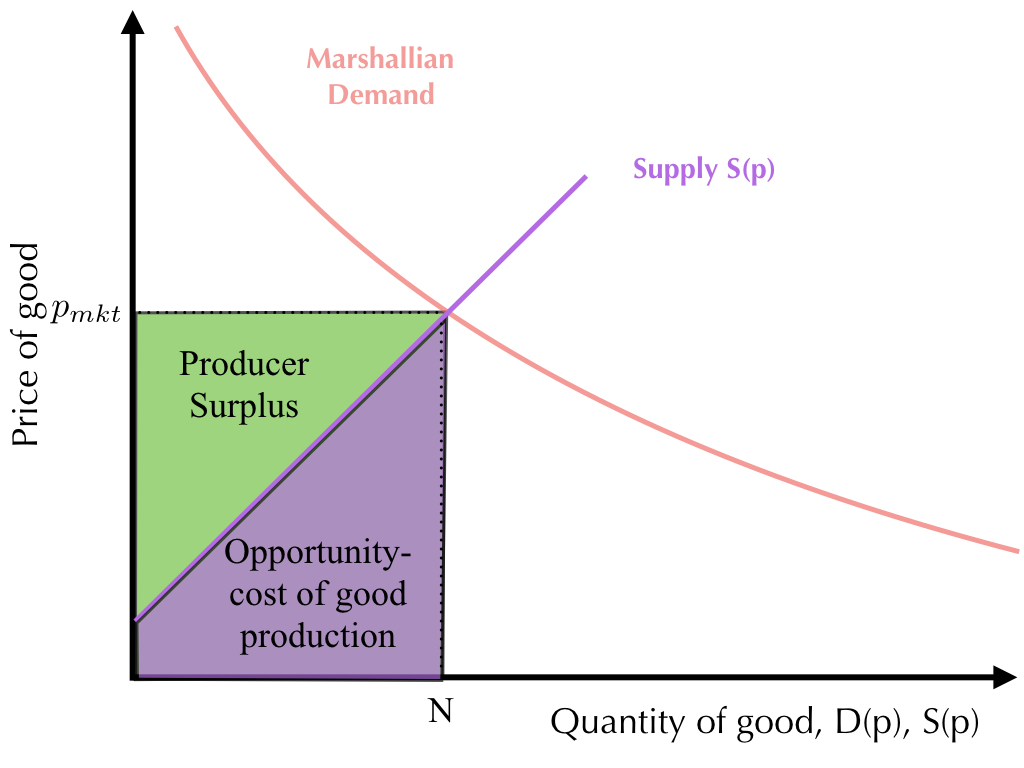
\includegraphics[width=0.5\linewidth]{Figures/PS2}
\end{figure}
{\footnotesize Left: Shaded area is total revenue received by supplier.}\\
{\footnotesize Right:PS is the total revenue for N goods minus the total opportunity cost of the resources employed for the production of N goods. The Supply gives the marginal opportunity cost of each unit of the good.}
\end{frame}


\begin{frame}{Computation}
\begin{figure}
	\centering
	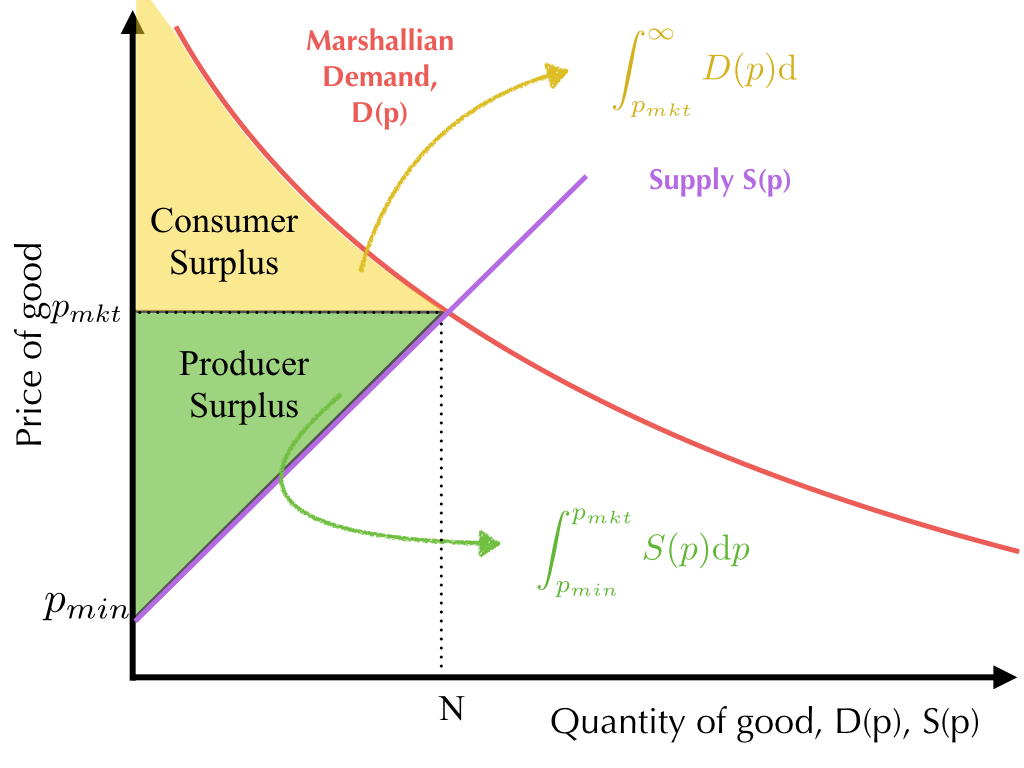
\includegraphics[width=0.7\linewidth]{Figures/SS}
\end{figure}
\end{frame}



\begin{frame}{CS and PS computations}
Denote the equilibrium price before a price change as $p_{mkt}$.

Consumer surplus is the region below the demand curve and above the price, and is equal to:\[\int_{p_{mkt}}^{\infty}D(p)\mathrm{d}p.\]

Let $p_{min}$ denote the price required to supply 0 units of the good. Producer surplus is the region below the market price and above the supply curve, and is equal to:\footnote{Usually $p_{min}=0$.}\[\int_{p_{min}}^{p_{mkt}}S(p)\mathrm{d}p.\]

\end{frame}

\begin{frame}{DWL from a Tax and Surplus Changes}
\begin{figure}
	\centering
	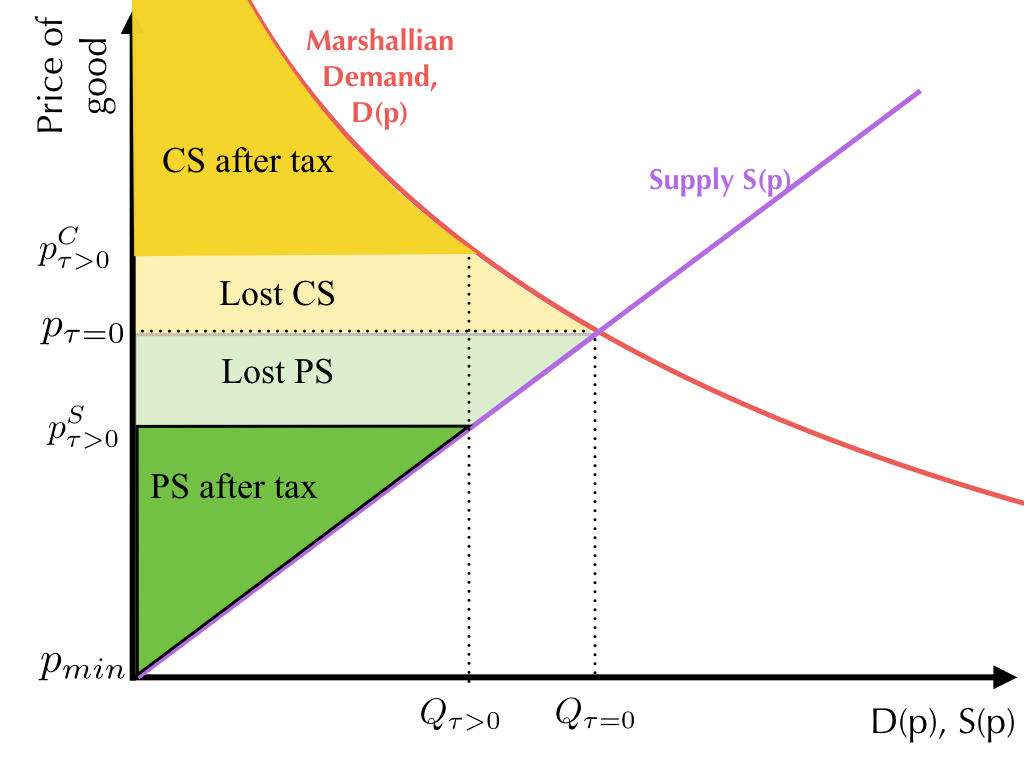
\includegraphics[width=0.5\linewidth]{Figures/Tax2}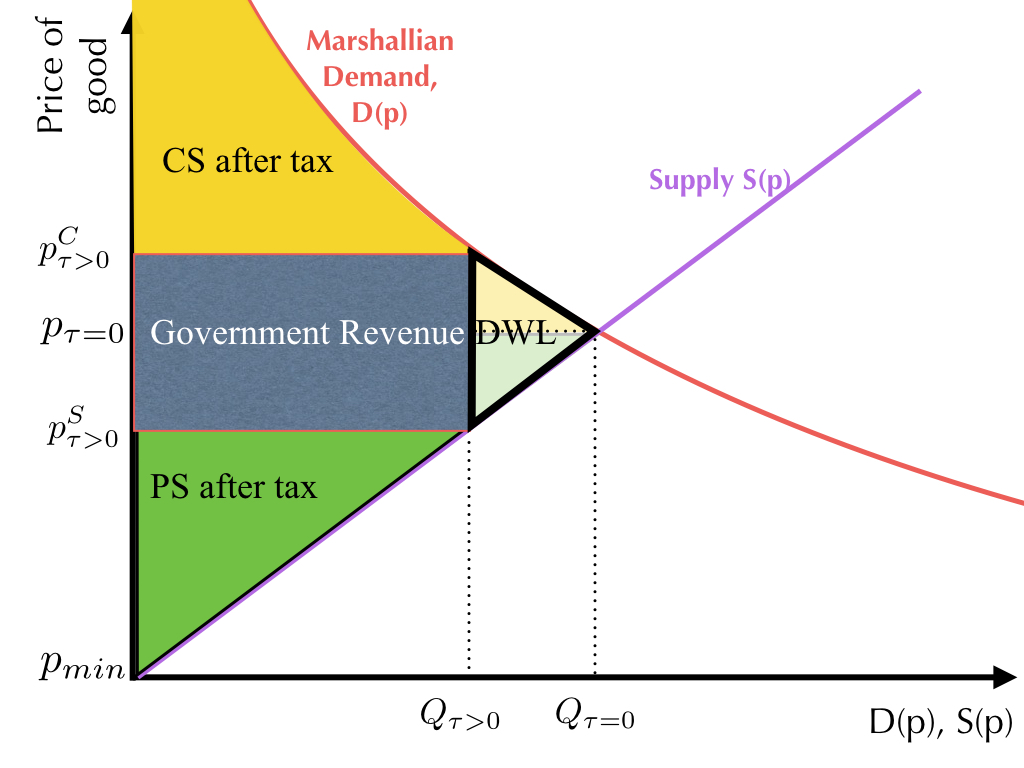
\includegraphics[width=0.5\linewidth]{Figures/Tax3}
\end{figure}
{\footnotesize Left: Lost CS is the area under the demand curve between the price after-tax and that before tax. Lost PS is the area above the supply curve between the price before tax  and that after-tax.}\\
{\footnotesize Right: Part of the lost surplus goes to the government in the form of tax revenues. DWL is given by the loss of efficient exchanges caused by the tax.}
\end{frame}

\begin{frame}{Surplus Change Computations and DWL}
Suppose that the tax changes the price paid by consumers (from $p_{\tau=0}$ to $p^{C}_{\tau>0}$) and received by suppliers (from $p_{\tau=0}$ to $p^{S}_{\tau>0}$). Then, the change in consumer surplus is:\[\Delta CS=\int_{p^{C}_{\tau>0}}^{\infty}D(p)\mathrm{d}p-\int_{p_{\tau=0}}^{\infty}D(p)\mathrm{d}p=\int_{p^{C}_{\tau>0}}^{p_{\tau=0}}D(p)\mathrm{d}p.\]

The change in producer surplus is:\[\Delta PS=\int_{p_{min}}^{p^{S}_{\tau>0}}S(p)\mathrm{d}p-\int_{p_{min}}^{p_{\tau=0}}S(p)\mathrm{d}p=\int_{p_{\tau=0}}^{p^{S}_{\tau>0}}S(p)\mathrm{d}p.\]
DWL is then given by:\footnote{For how we wrote the integrals, this quantity is negative, but this is just a convention, we could flip all signs and write DWL as a positive quantity (absolute value).}
\[ DWL=\Delta CS + \Delta PS + \text{Government Revenue}. \]


\end{frame}



\begin{frame}{DWL Depends Only on Quantity Adjustments\dots}
\begin{figure}
	\centering
	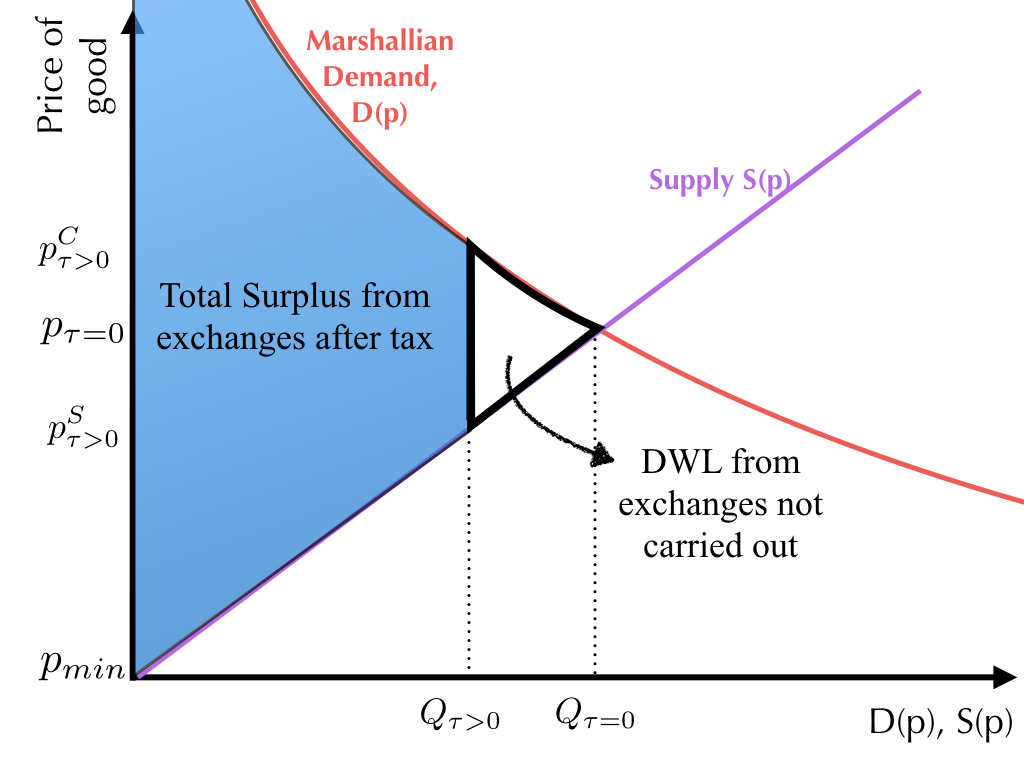
\includegraphics[width=0.5\linewidth]{Figures/Tax4}
\end{figure}
{\footnotesize DWL comes from lost exchanges, prices only determine how this loss is shared by consumers versus producers. Of course the size of the DWL will depend on the smallest elasticity across the two agents. If any of the two parties is fully inelastic, there is no DWL.}
\end{frame}


\begin{frame}{\dots but Incidence Depends on Relative Elasticity}

Remember the inverse elasticity formula. With demand and supply:
\[
	D(p) = p^{-\eta}, \ S(p) = p^\varepsilon,
\]
the tax burden on consumer is:
\[
	\dfrac{\varepsilon}{\eta + \varepsilon}\tau,
\]
and on producer is:
\[
\dfrac{\eta}{\eta + \varepsilon}\tau.
\]
Finally, if you have a percent tax, so that:
\[
	p^C = (1+\tau)p^S,
\]
the percent change in quantity, which determines the DWL, is approximately:
\[
	\%\Delta Q= -\dfrac{\eta \varepsilon}{\eta + \varepsilon}\tau.
\]

\end{frame}



\section{General Equilibrium: Pure Exchange}

\begin{frame}{General Equilibrium in Pure Exchange}
A General Equilibrium is a set of \textbf{prices} $\left\lbrace p_1, p_2\right\rbrace$, and \textbf{allocations} for consumption  $\left\lbrace \underline{c}_1, \underline{c}_2\right\rbrace$ such that, given initial endowments of goods $\underline{e}_1, \underline{e}_2$:
\begin{enumerate}
	\item Consumers choose consumption $\left\lbrace \underline{c}_1, \underline{c}_2\right\rbrace$ subject to their budget constraint for given \textbf{prices};
	\item  The good markets clear.
\end{enumerate}
\end{frame}



\begin{frame}{Solving GE}
		\begin{enumerate}
			\item Technology $\Rightarrow$ PPF (in pure exchange this is just given by the endowments);
			\item Preferences $\Rightarrow$ Indifference curves;
			\item  Endowments with 1 and 2 $\Rightarrow$ price ratio.
		\end{enumerate}
\end{frame}

\begin{frame}{Solving GE in Pure Exchange}
GE is given by the point \textbf{in the Edgeworth box} such that indifference curves are tangent to each other and utility is maximized for given initial endowments, and the price ratio that is tangent to the indifference curves.\\
Steps:
\begin{enumerate}
	\item Solve the consumer problem for given income $I$ for both consumers;
	\item For each consumer, set $I = p_1e_1 + p_2e_2$, find $c_1, c_2$ as a function of price ratio;
	\item Impose market clearing: $c^1_1 + c^2_1 = e^1_1 + e^2_1 = E_1$.\footnote{Superscripts denote the agent's identity, subscripts the goods.}
\end{enumerate}
\end{frame}

\begin{frame}{Edgeworth Box: An example}
Consider an economy with two goods, x and y, and two agents, A and B, with preferences:
\begin{equation}\label{Ua}
U^A(x^A, y^A) = x^A\times y^A,
\end{equation}
\begin{equation}\label{Ub}
U^B(x^B, y^B) = (x^B)^\frac{2}{3}\times(y^B)^\frac{1}{3},
\end{equation}
denote the price ratio $p_y/p_x \equiv p$ (level does not matter), and let the total endowments of goods be $X = 10, Y=10$, and denote individual endowments by $e_{good}^i$ for $good$ in $\left\lbrace x, y \right\rbrace$ and $i$ in $\left\lbrace A, B \right\rbrace$. 

The budget constraint for each agent $i$ is then:
\begin{equation}\label{BC}
x^i + py^i = I^i = e_x^i + pe_y^i
\end{equation}

The general equilibrium of this economy is an allocation $\left\lbrace x^A, y^A, x^B, y^B \right\rbrace$ and a price $p$, such that $\left\lbrace x^A, y^A\right\rbrace$ and $\left\lbrace x^B, y^B\right\rbrace$ maximize \eqref{Ua}, \eqref{Ub} subject to \eqref{BC}, and markets clear, that is:
\[
	x^A + x^B = e_x^A + e_x^B = X, \ \ y^A + y^B = e_y^A + e_y^B = Y
\]
\end{frame}


\begin{frame}{Example Solution}

\end{frame}



\begin{frame}{Edgeworth Box: Indifference curves for A and B}
\begin{figure}
	\centering
	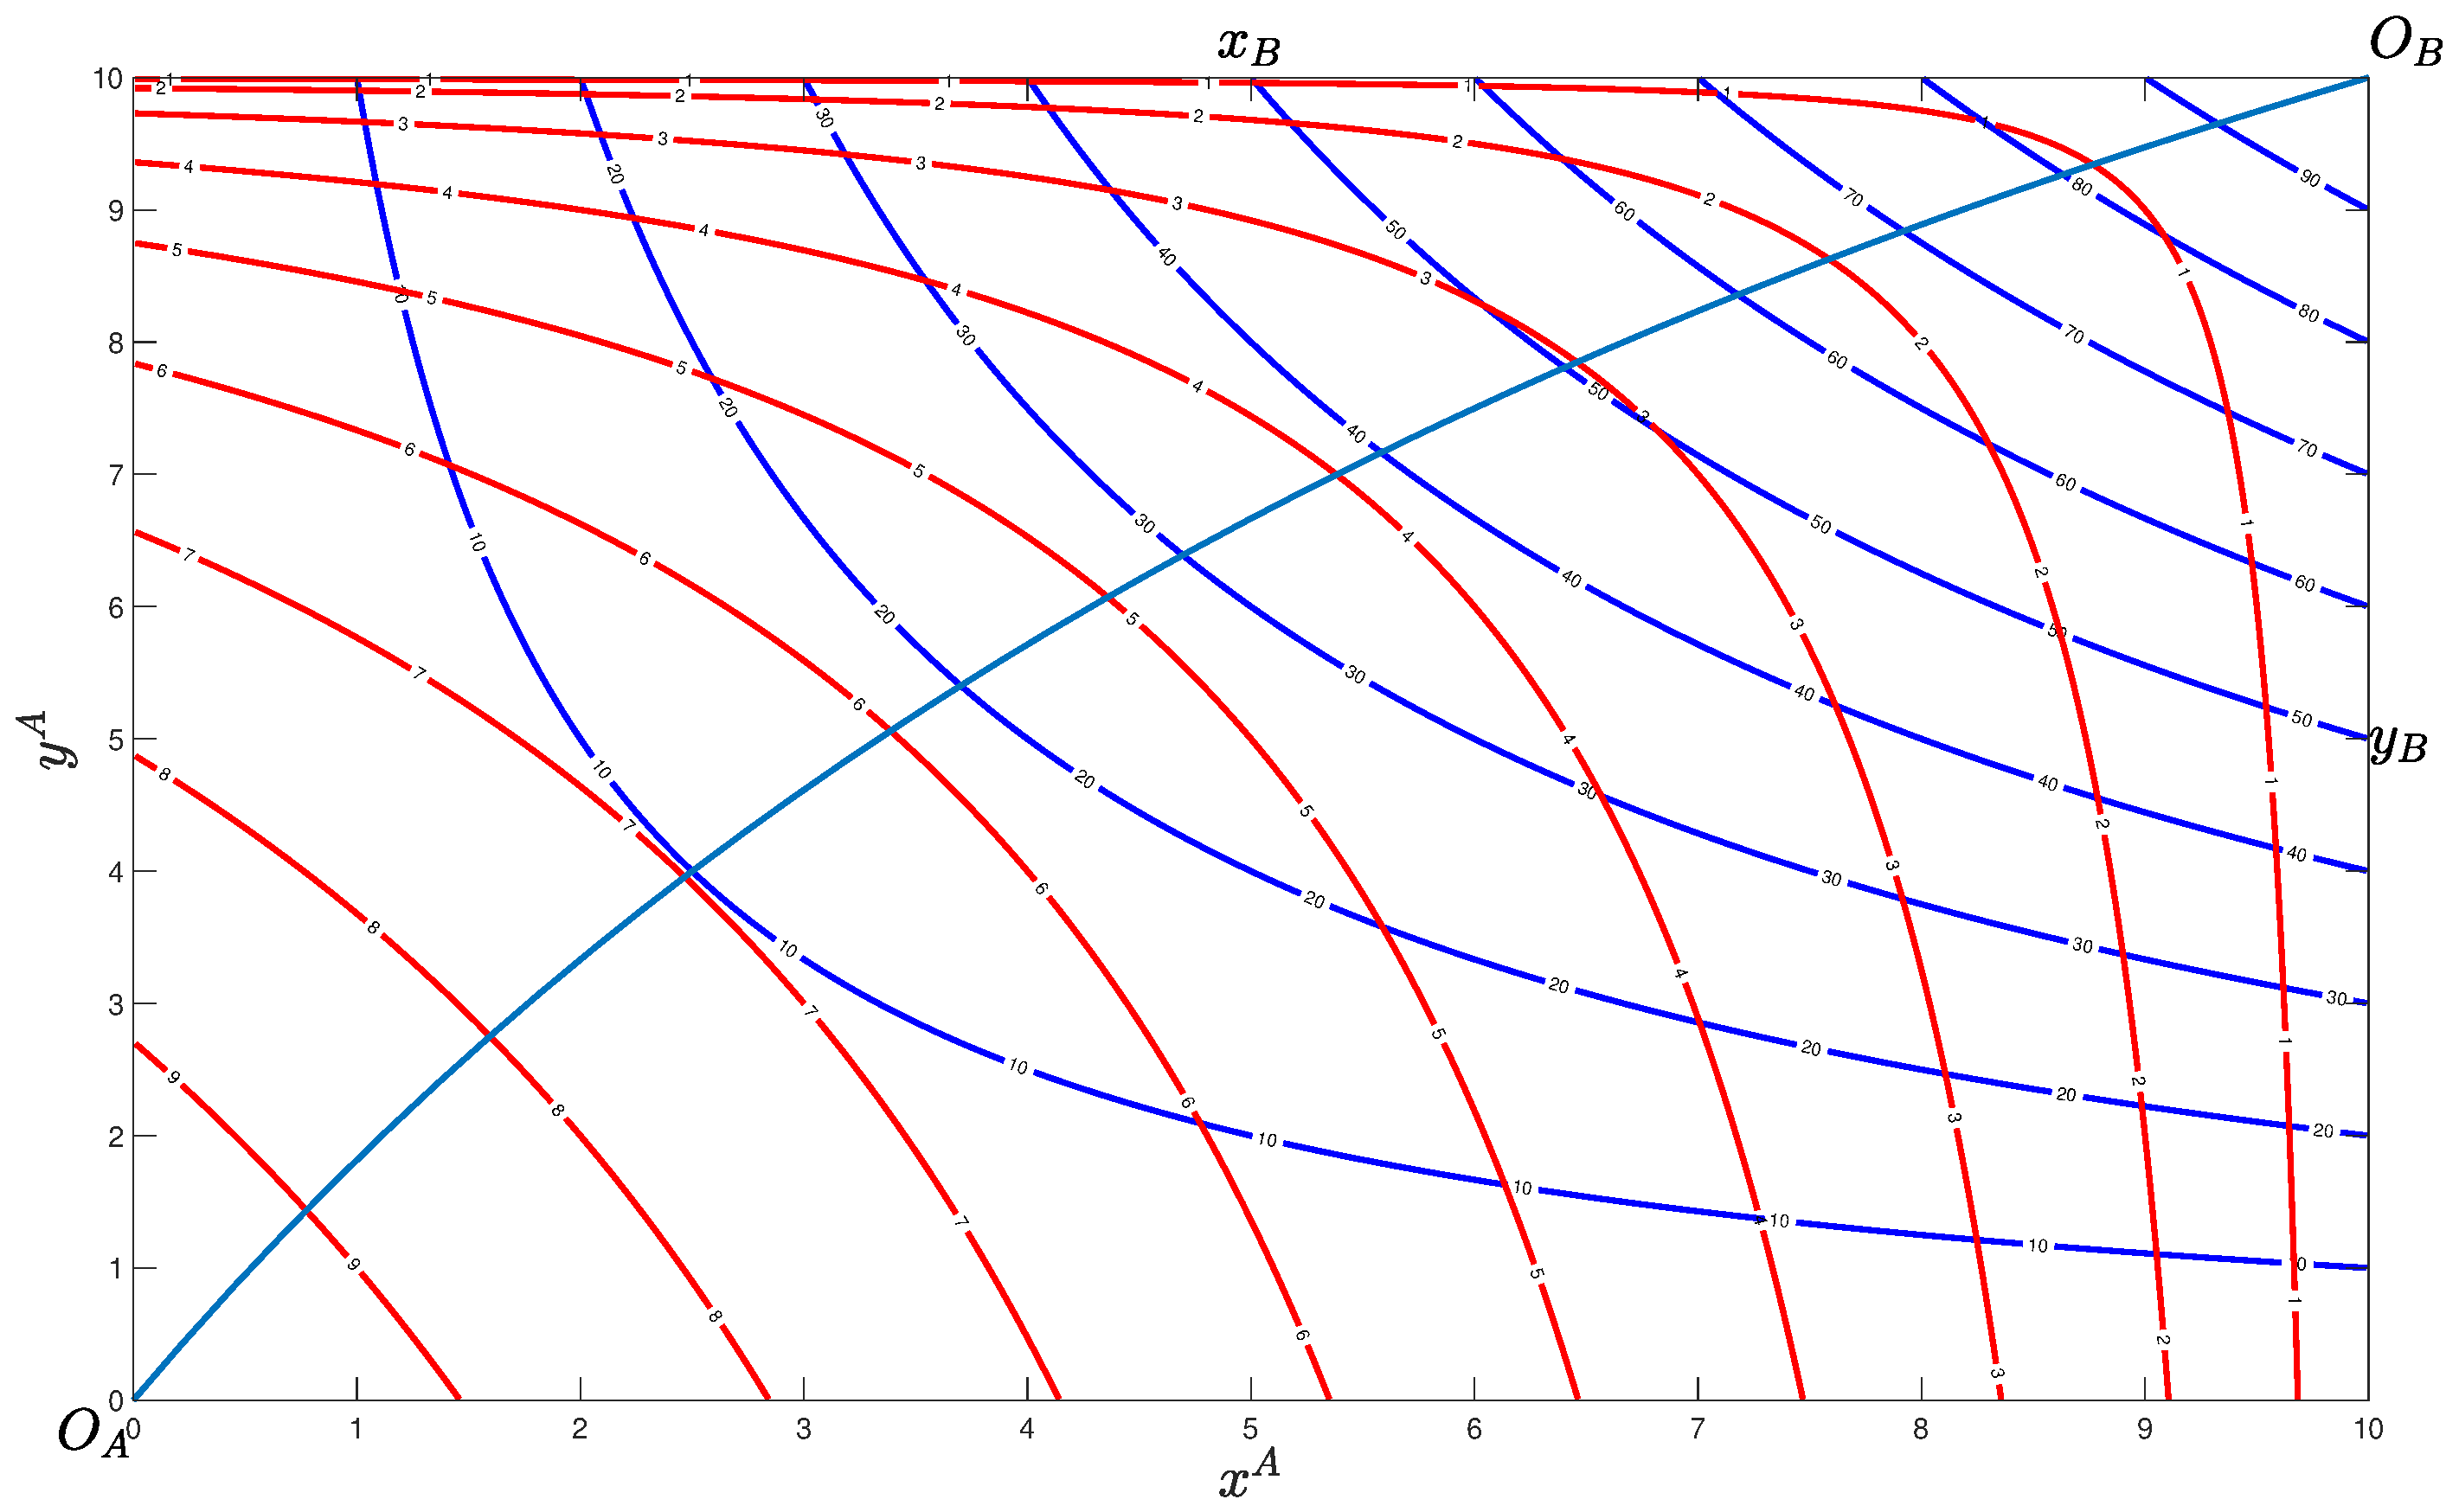
\includegraphics[width=0.7\linewidth]{Figures/Edgeworth_3}
\end{figure}


\end{frame}






\begin{frame}{GE with Production in Autarky: Equilibrium}
\begin{figure}
	\centering
	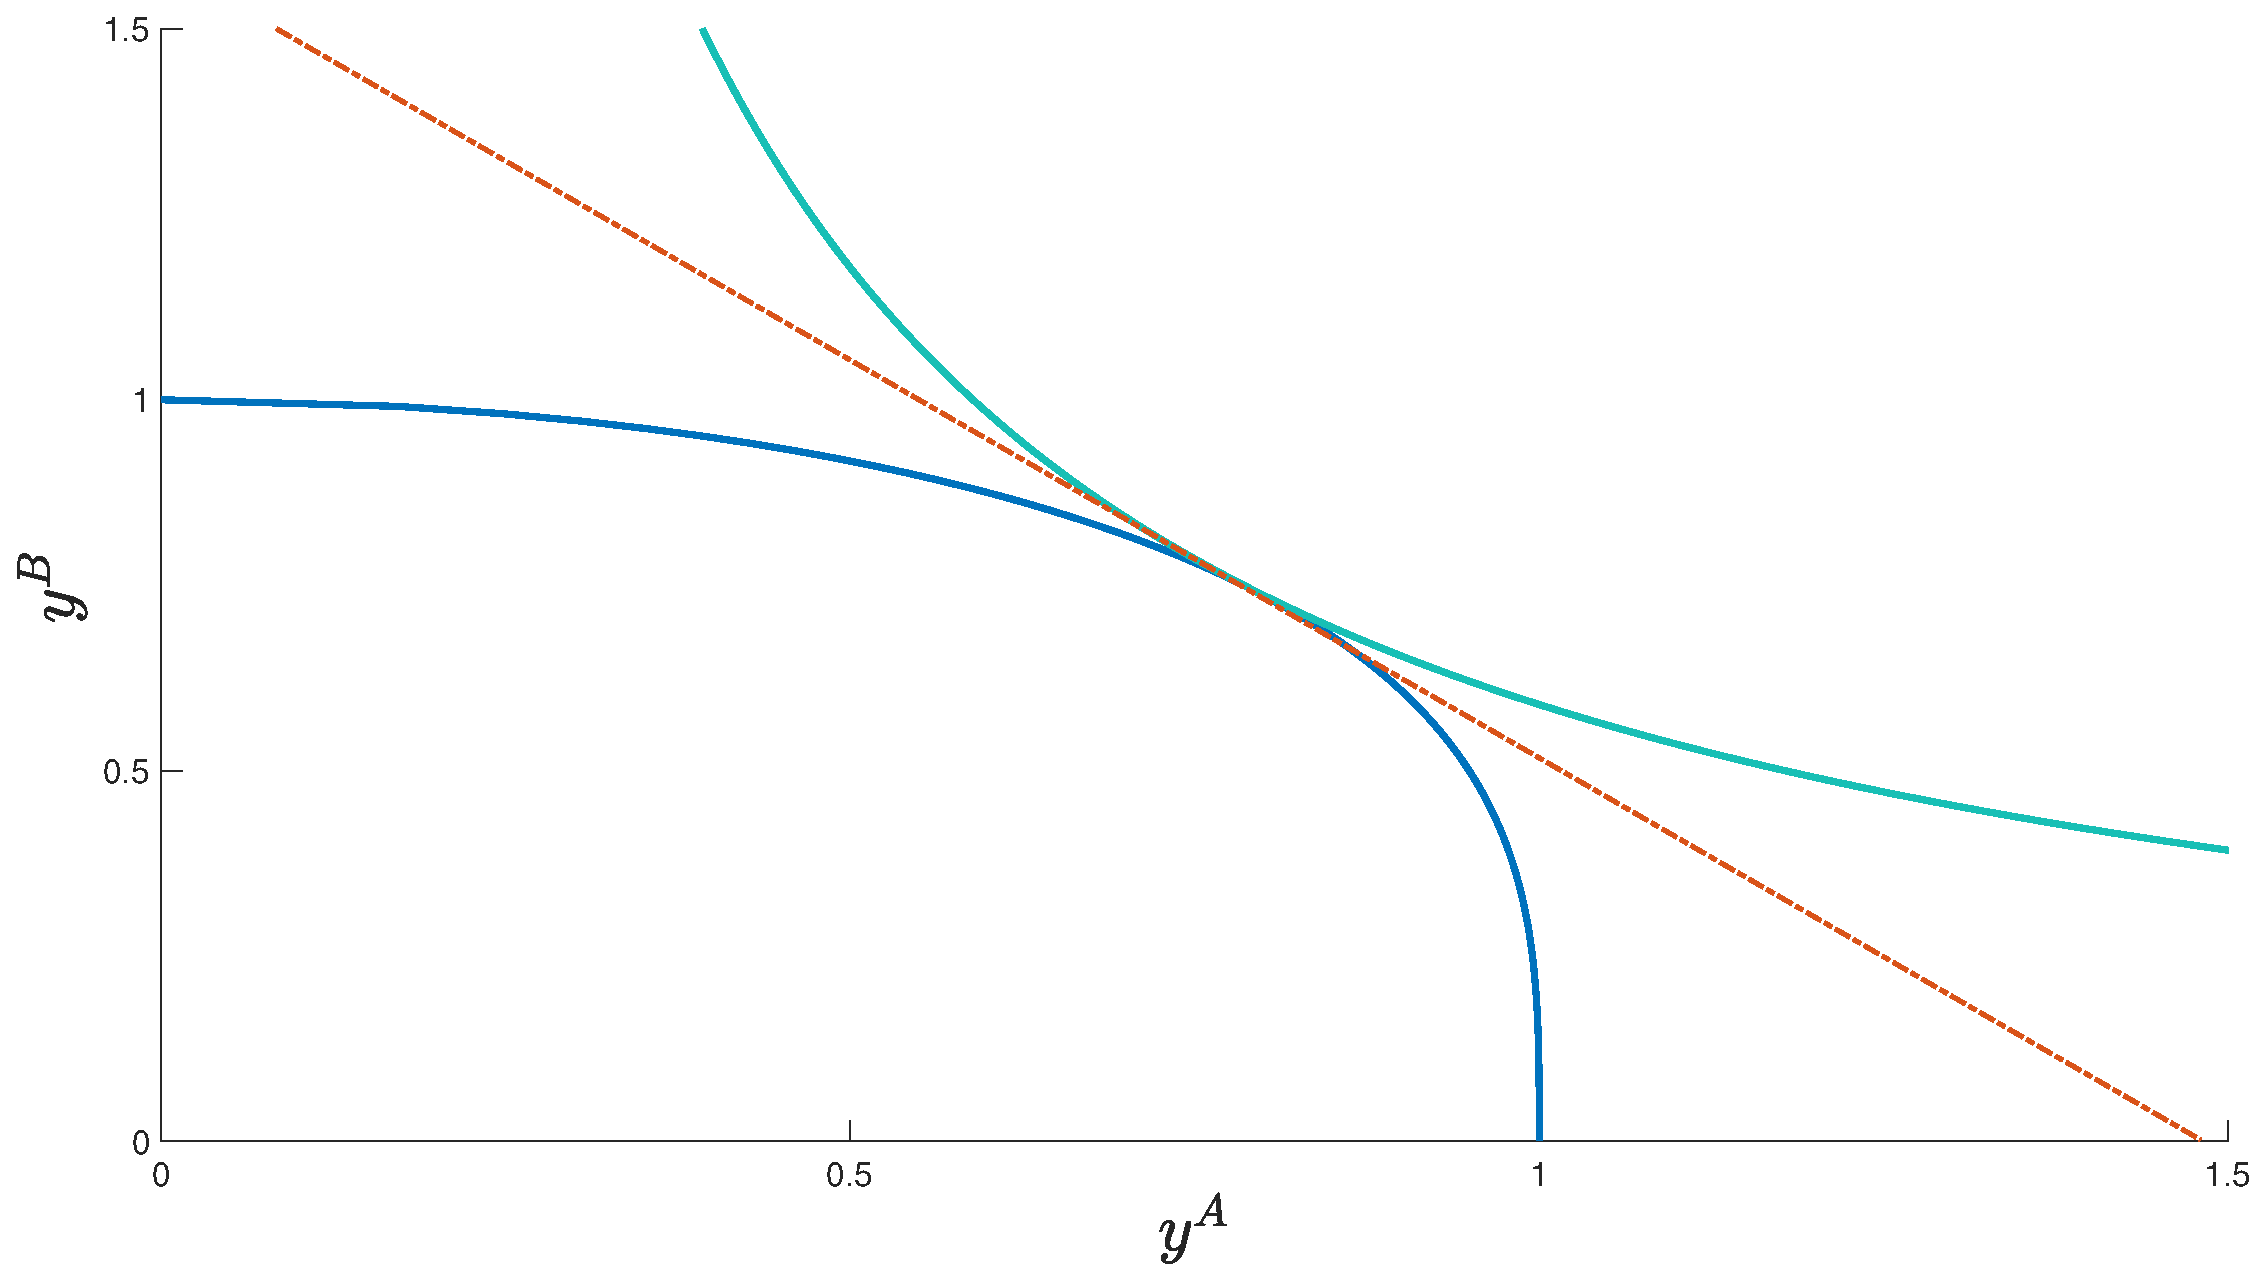
\includegraphics[width=0.7\linewidth]{Figures/PPF}
\end{figure}

\end{frame}



\section{Gains from International Trade}

\begin{frame}{Trade as Constraint-Relaxation}
	\begin{itemize}
		\item A Pareto-Improvement will be realized when trade relaxes a constraint.
		\item Within-country trade always generates a Pareto-improvement \textit{relative to endowment consumption}. \textit{The relaxed constraint is consuming \textbf{one's own endowment}, now all trades starting from it are possible}.
		\item International trade always generates a Pareto-improvement \textit{relative to production in autarky without within-country exchange}. \textit{The relaxed constraint is consuming along the PPF  \textbf{at domestic price ratio}, now all trades starting from it are possible. Moreover, gains from specialization and comparative advantage}.
		\item \textit{However}, international trade does not \textit{always} generate a Pareto-improvement \textit{relative to within-country exchange}. Allocation before: pure exchange economy between different parts of the economy. Allocation after: trade with abroad at different price ratio.
		\item In the last case, agents that are endowed with more of the relatively expensive good benefit gain, while those with more of the relatively cheap good lose (see ADH Figure in next slides).
		
	\end{itemize}
\end{frame}


\begin{frame}{International trade versus endowment}
\begin{figure}
	\centering
	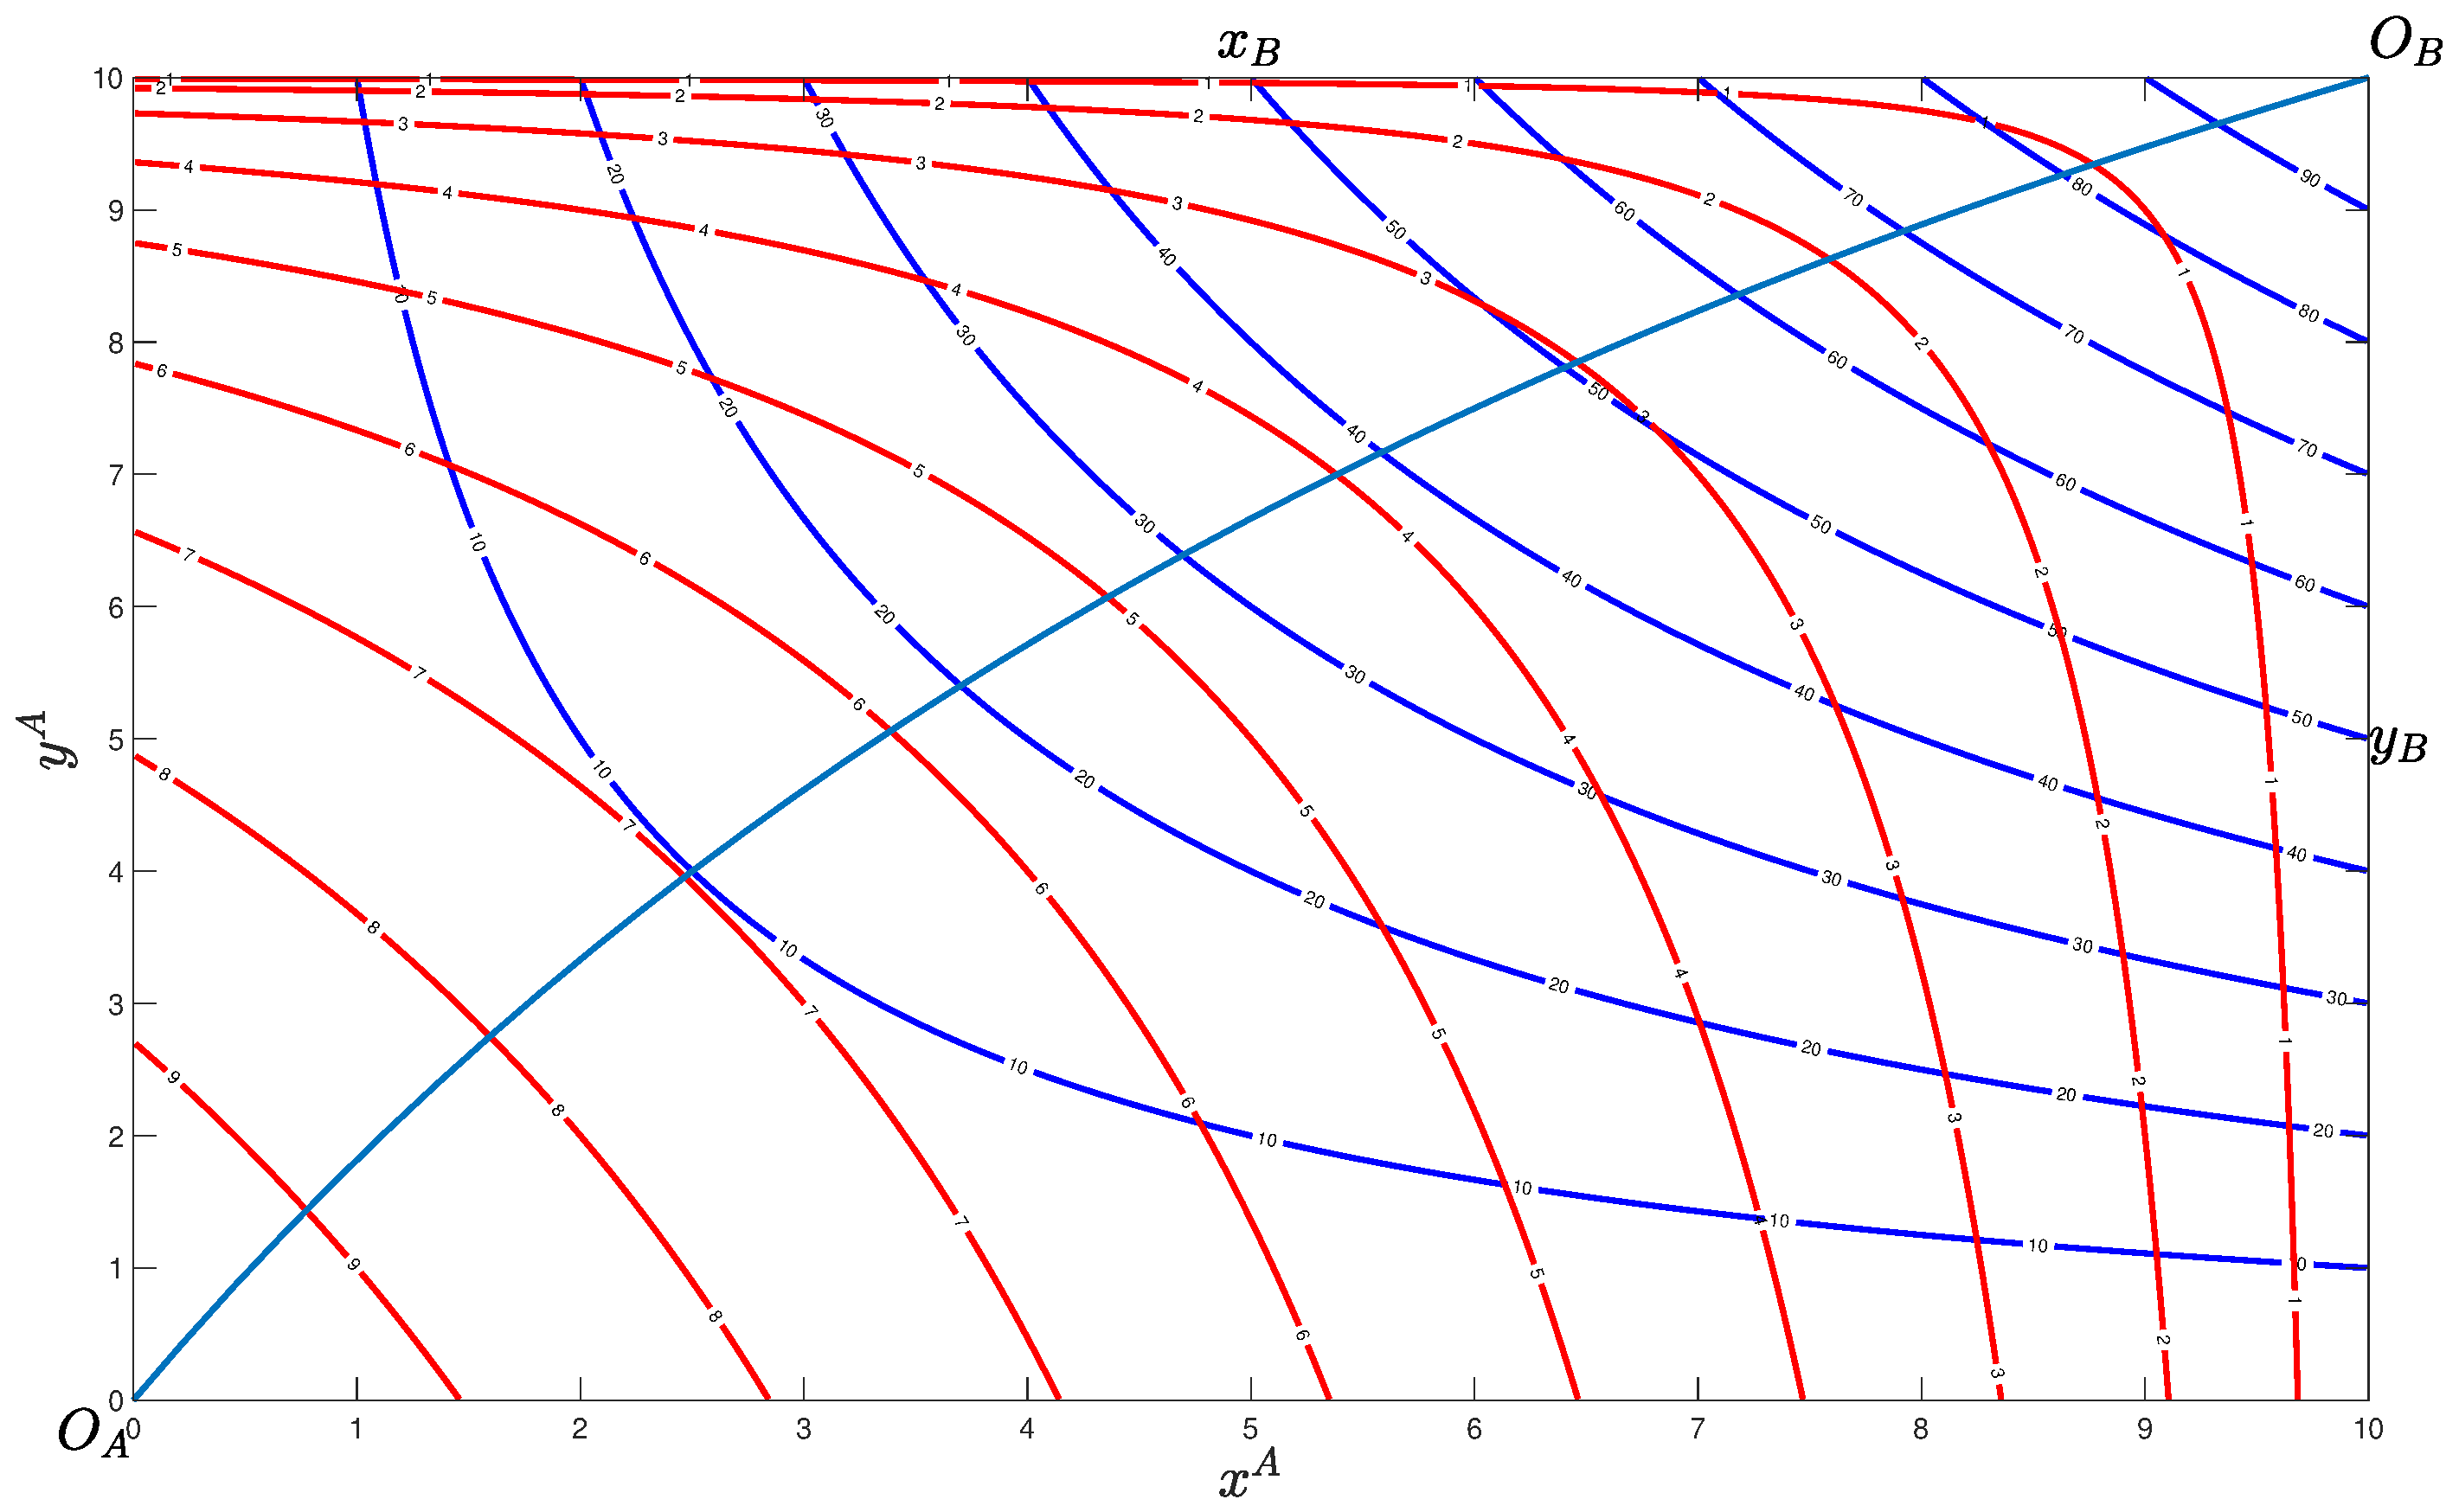
\includegraphics[width=0.7\linewidth]{Figures/Edgeworth_3}
\end{figure}


\end{frame}


\begin{frame}{GE with Production: Trade}
\begin{figure}
	\centering
	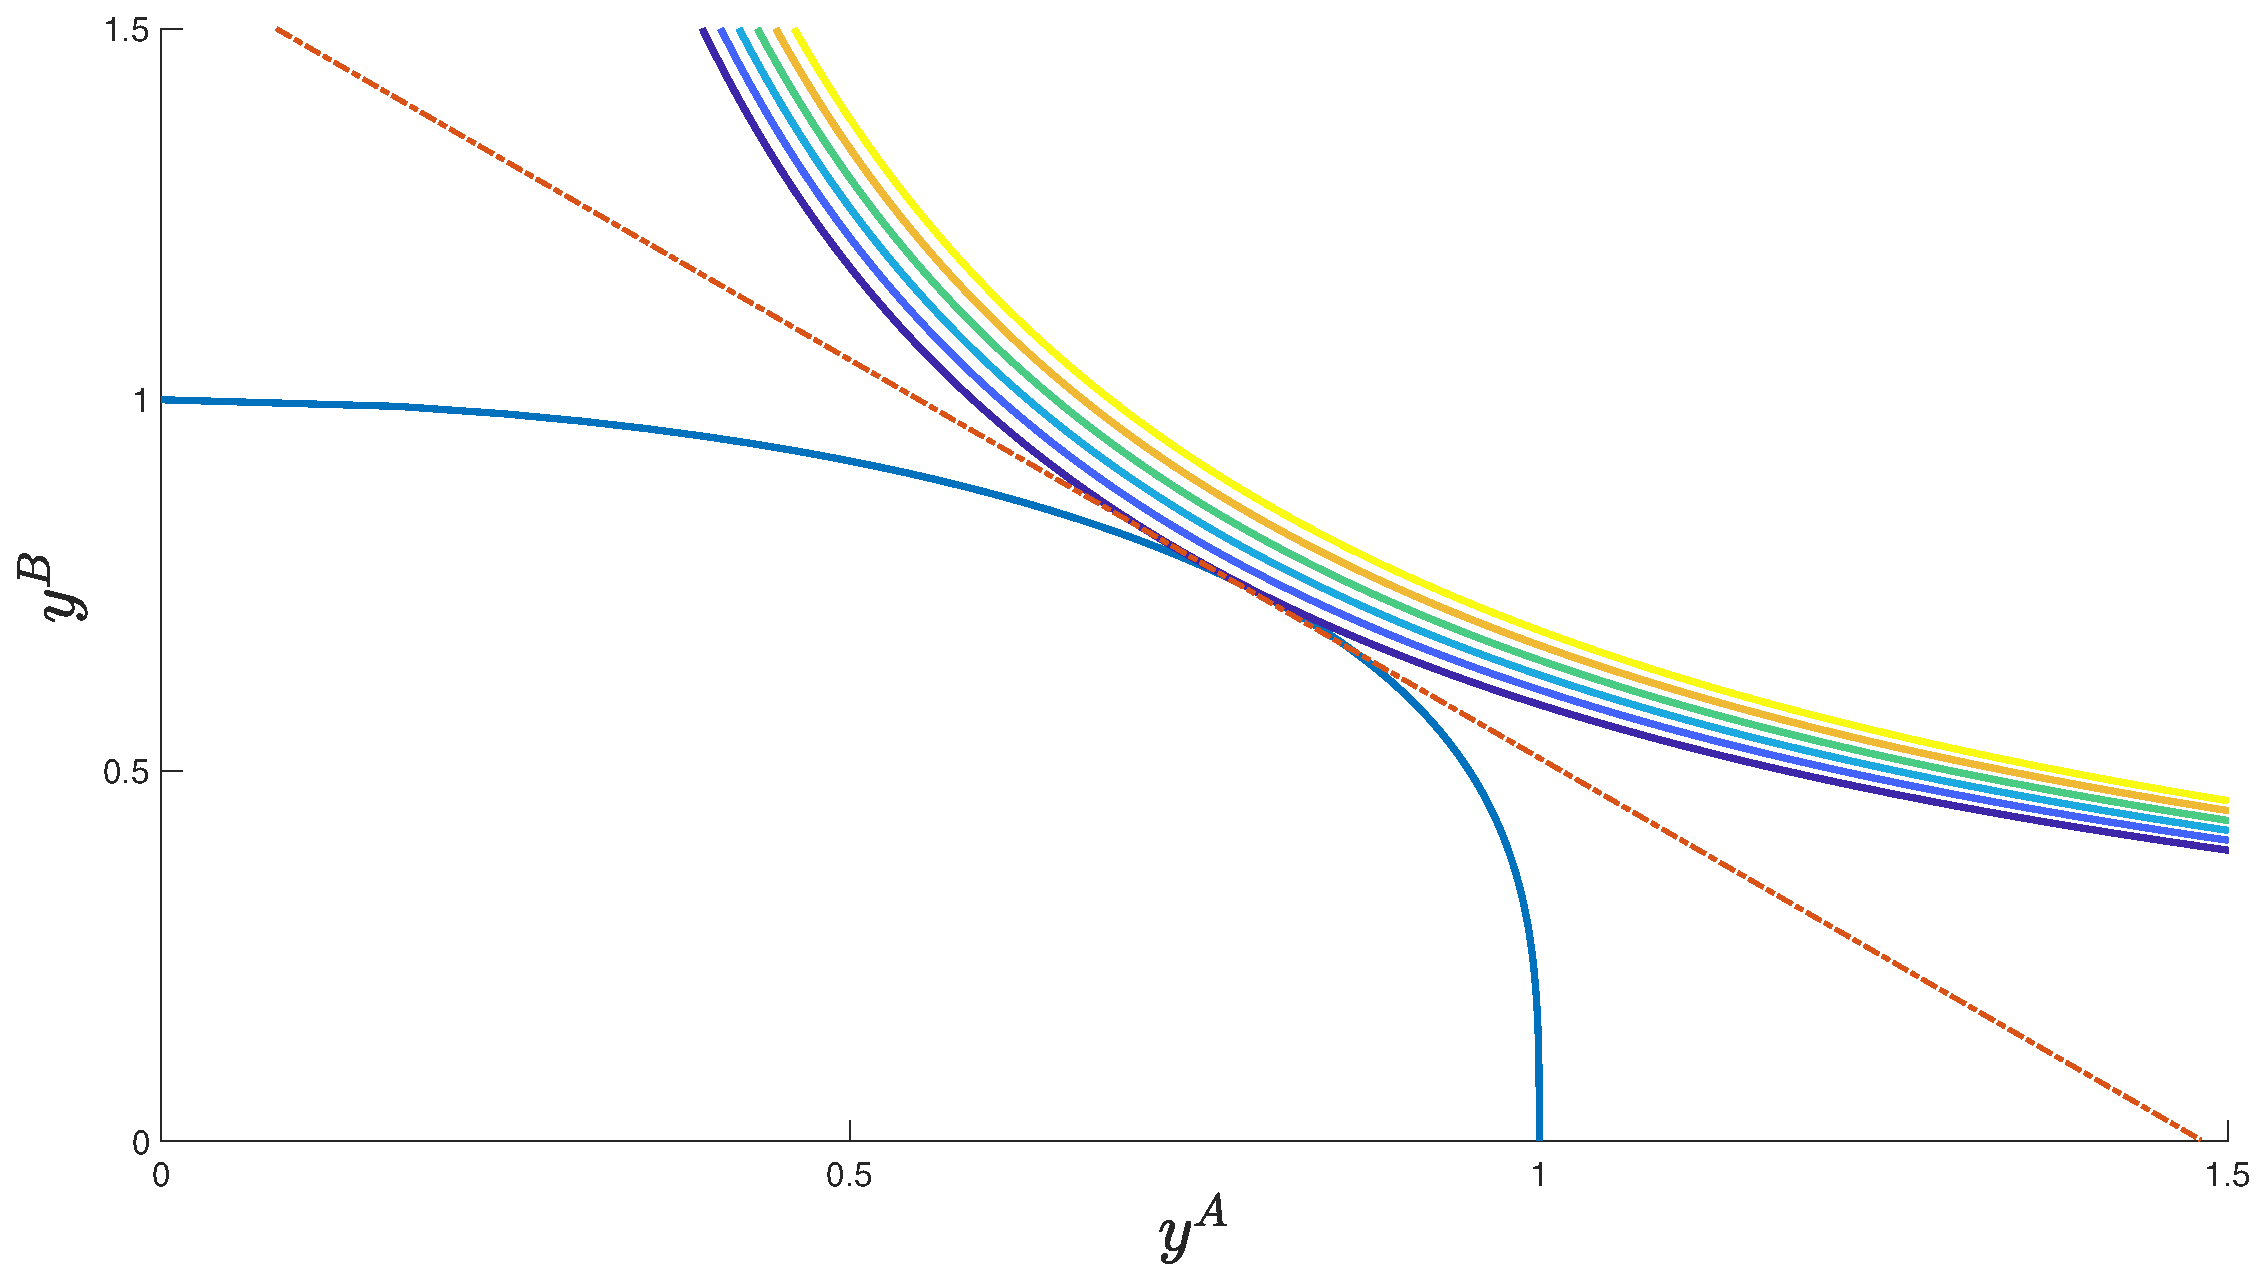
\includegraphics[width=0.7\linewidth]{Figures/PPF_2}
\end{figure}
{\footnotesize Gains arise if the country has comparative advantage relative to abroad. That is,
	\[\left(\frac{p^A}{p^B}\right)_{\text{Autarky}}\neq\left(\frac{p^A}{p^B}\right)_{\text{Trade}}.
	\] }
\end{frame}



\begin{frame}{International versus Within-Country Trade}
\begin{figure}
	\centering
	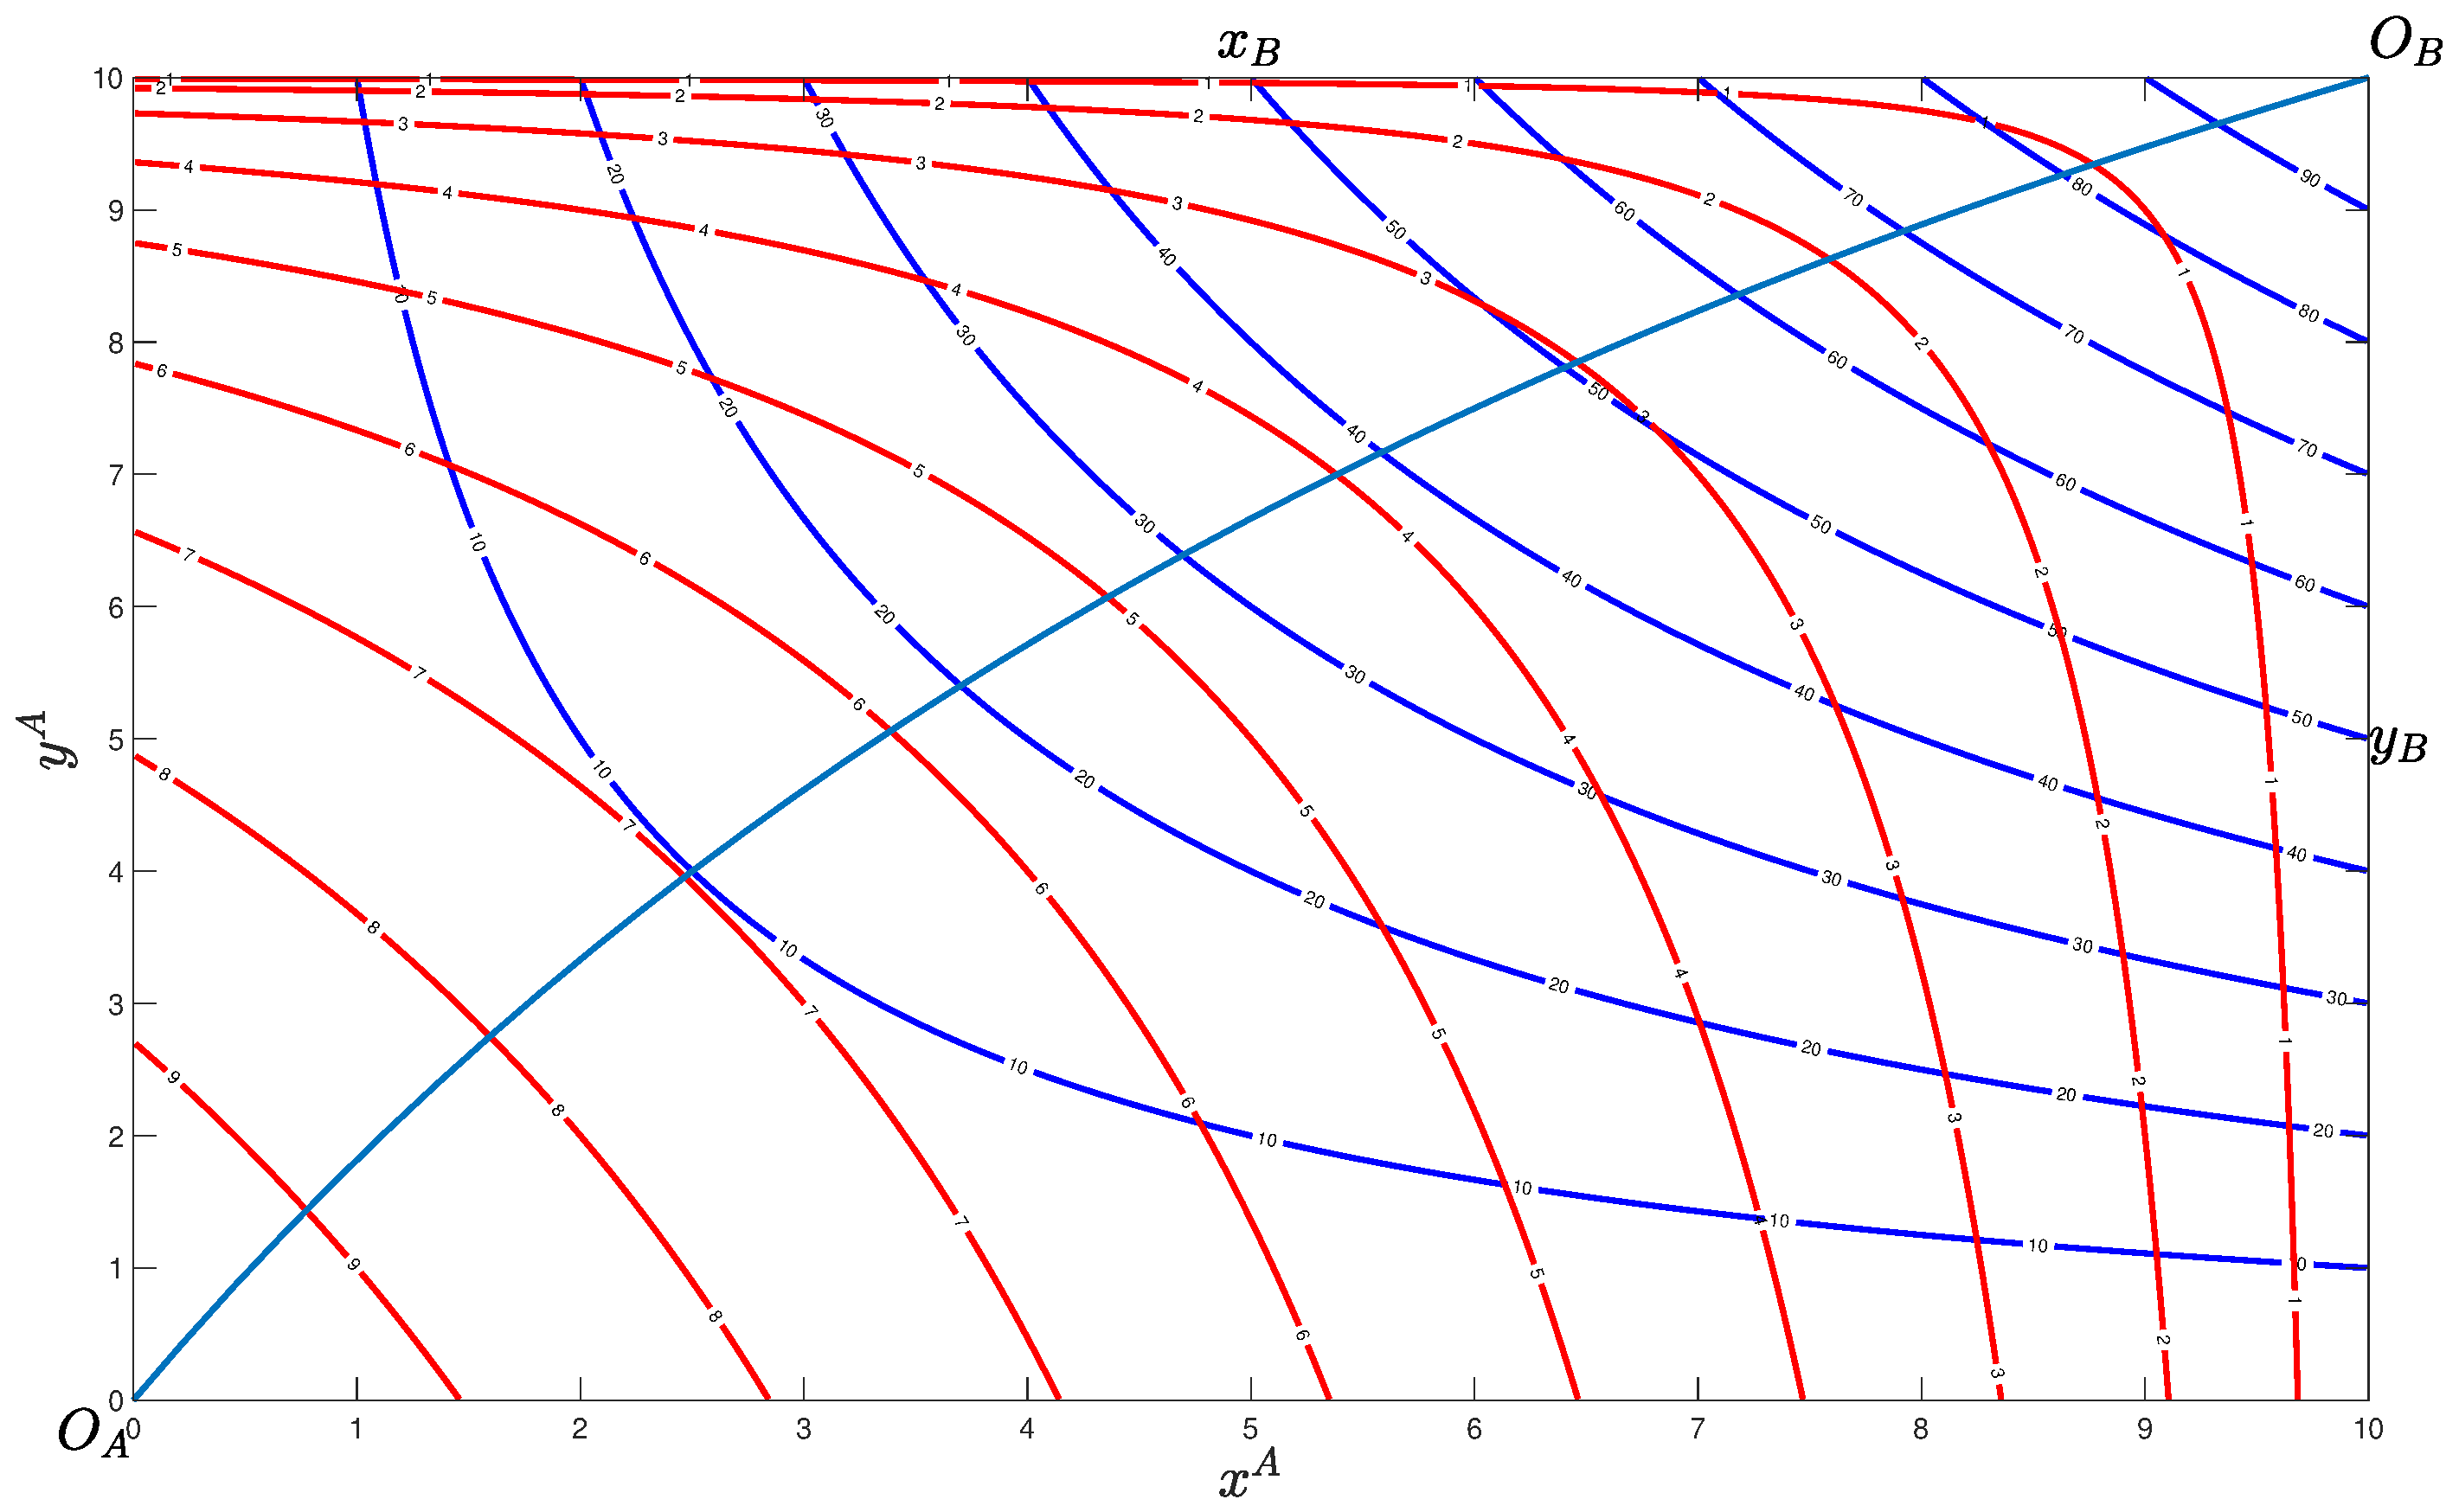
\includegraphics[width=0.8\linewidth]{Figures/Edgeworth_3}
\end{figure}
\end{frame}

\begin{frame}{International versus Within-Country Trade II}
\begin{figure}
	\centering
	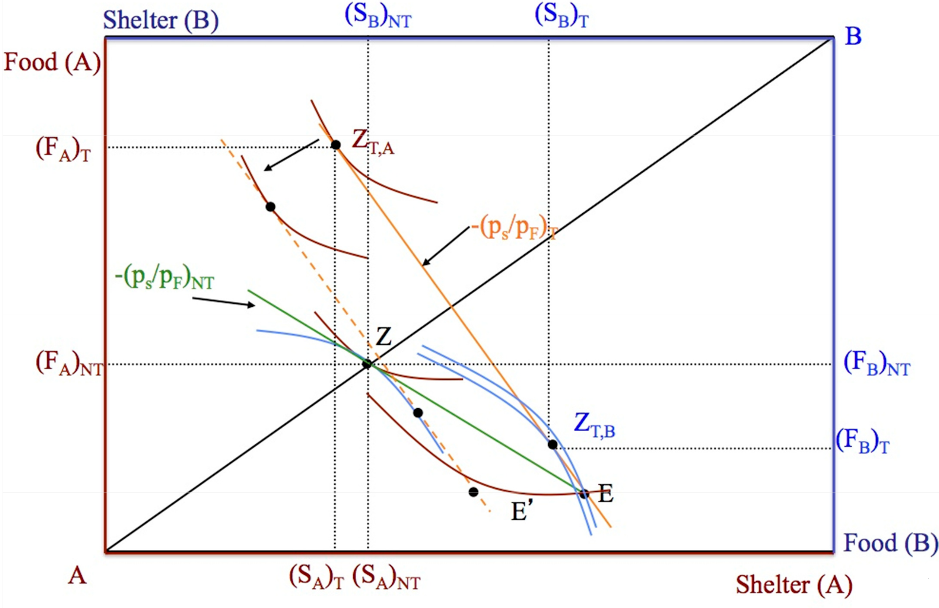
\includegraphics[width=0.8\linewidth]{Figures/TradeDistribution}
\end{figure}
\end{frame}


\begin{frame}{May L\'{e}on Walras be with you\dots}
\begin{figure}
	\centering
	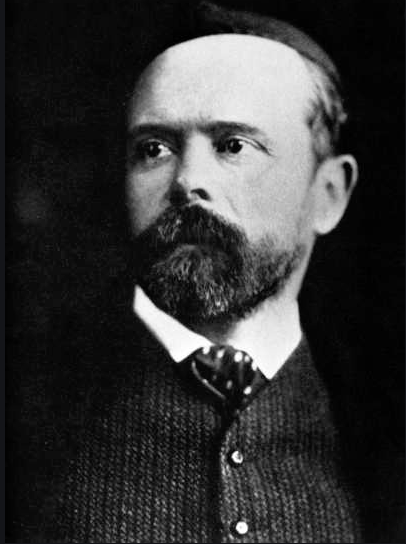
\includegraphics[width=0.5\linewidth]{Figures/walras_pic}
	\label{fig:walraspic}
\end{figure}
\end{frame}